%
% Documento: FRAMEWORK PROPOSTO
%
\chapter{ARQUITETURA DO PYBOT}\label{chap:imp}
    O \emph{framework} consiste em alguns módulos básicos, cada um com suas devidas utilidades e funções.
    A separação dos de cada módulos foi dada com base em suas características e funcionalidades.

    Na Figura \ref{fig:modules}, apresenta-se a solução modular composta pelos módulos e as classes principais do
    \emph{framework} e nas próximas seções serão detalhados cada um deles.


    \begin{figure}[H]
        \vspace*{0,3cm}
        \centering
        \caption{Diagrama de Componentes}
        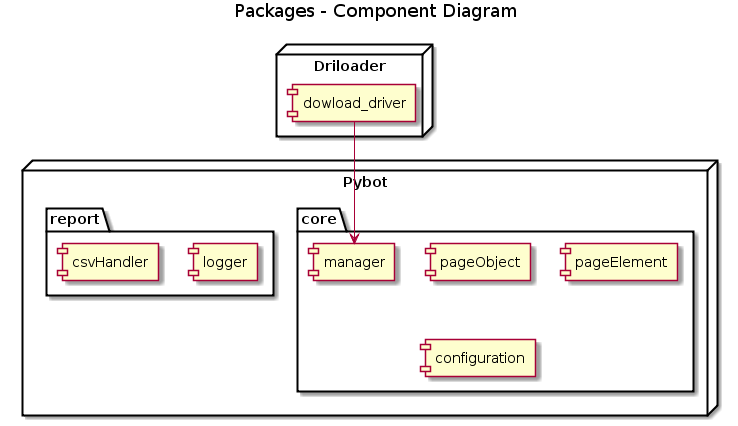
\includegraphics[width=1\textwidth]{./04-figuras/model}
        \label{fig:modules}
    \end{figure}
    \vspace*{-0,9cm}
    {\raggedright \fonte{Autor desta monografia, 2017.}}



    \section{Core}
        Este módulo contém as funcionalidades básicas para a operação do \emph{framework} com o Selenium \emph{Webdriver}
        e o gerenciamento dos parâmetros de execuções de cada \emph{script}.

        \subsection{Manager} \label{sec:manager}
        A classe \emph{Manager} serve para abstrair o uso do Selenium \emph{Webdriver} criando uma camada de métodos próprios fazendo com que caso alguma
        atualização da API do Selenium \emph{Webdriver} altere os \emph{scripts} criados não sejam impactados. Fazendo uso do Driloader mencionado na
        subseção \ref{driloader} ele verifica a necessidade do download do \emph{driver} para poder executar o \emph{Selenium Webdriver}.

        Como exemplo na Figura~\ref{fig:manager} temos o exemplo de alguns dos comando disponíveis do Manager, sendo o da linha 4 para o inicio do processo
        e execução do \emph{driver} do navegador, na linha 7 para navegar para uma URL e na linha 12 para finalizar o processo.

        \begin{figure}[H]
            \vspace*{0,3cm}
            \centering
            \caption{Exemplo - Uso da classe Manager}
            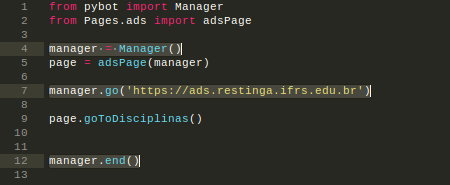
\includegraphics[width=0.8\textwidth]{./04-figuras/manager}
            \label{fig:manager}
        \end{figure}
        \vspace*{-0,9cm}
        {\raggedright \fonte{Autor desta monografia, 2017.}}

        \subsection{Configuration}
        Responsável por gerar as configurações básicas para o \emph{framework} e disponibilizá-las no arquivo \emph{pybot.ini}.
        Este arquivo é criado automaticamente para cada script do usuário e nele é possível adicionar qualquer tipo de configurações ou parâmetros
        necessários para a execução do \emph{script}.

        Como exemplo, pode ser observado na linha 8 da código apresentado na Figura~\ref{fig:config} o comando base para buscar uma determinada configuração do arquivo.

        \begin{figure}[H]
            \vspace*{0,3cm}
            \centering
            \caption{Exemplo - Uso do Configuration}
            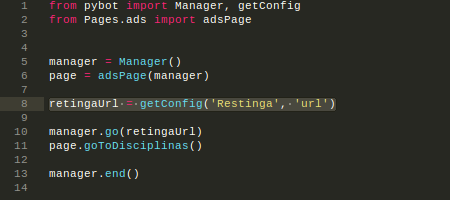
\includegraphics[width=0.8\textwidth]{./04-figuras/config}
            \label{fig:config}
        \end{figure}
        \vspace*{-0,9cm}
        {\raggedright \fonte{Autor desta monografia, 2017.}}

        O padrão de escrita das configurações pode ser visto na \autoref{fig:pybot.ini}, onde é necessário ter uma Seção e as variáveis desejadas.
        E para a utilização delas segue o mesmo padrão: \\ \mbox{\emph{configuration.getConfig('Seção', 'variável')}}.

        \begin{figure}[H]
            \vspace*{0,3cm}
            \centering
            \caption{Estrutura pybot.ini}
            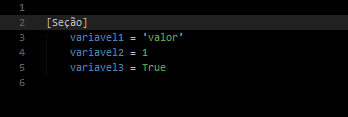
\includegraphics[width=0.7\textwidth]{./04-figuras/ini}
            \label{fig:pybot.ini}
        \end{figure}
        \vspace*{-0,9cm}
        {\raggedright \fonte{Autor desta monografia, 2017.}}



    \section{Component} \label{sec:comp}
        Módulo criado para seguir os padrões de \emph{PageObject} e \emph{PageElement}, contendo as classes de PageObject e PageElement e a classe responsável
        pela abstração para o \emph{WebElement} do \emph{Selenium Webdriver}.

        Pode-se observar na Figura \ref{fig:eleme} o uso das classes \emph{PageObject}, \emph{PageElement} e \emph{PageElements} nas linhas 3, 4 e 5 respectivamente.

        \begin{figure}[H]
            \vspace*{0,3cm}
            \centering
            \caption{Exemplo - Uso PageObject com PageElement e PageElements}
            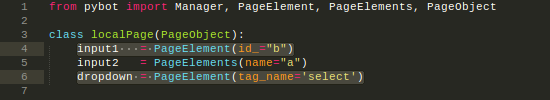
\includegraphics[width=1\textwidth]{./04-figuras/pageElement}
            \label{fig:eleme}
        \end{figure}
        \vspace*{-0,9cm}
        {\raggedright \fonte{Autor desta monografia, 2017.}}

        \subsection{WebElement}
            Serve para abstrair o uso da classe \emph{WebElement} do próprio \emph{Selenium Webdriver}. Contendo uma classe para cada tipo de campo dos \emph{html},
            ele dispõe de algumas funcionalidades básica, como a atribuição de uma valor para um elemento do tipo \emph{input text} irá escrever
            valor dentro do campo, \emph{select} irá selecionar a opção cujo texto seja igual ao valor informado, \emph{radio} irá selecionar o
            a opção que tenha o \emph{value} do valor informado e para o tipo \emph{checkbox} irá marcar ou desmarcar as opções se o valor for
            verdadeiro(\emph{True}) ou falso(\emph{False})

        \subsection{PageElement e PageElements}
        \label{PageElement}
            Essas classes servem para controlar os elementos mapeados das telas. Sempre quando serão acessadas a classe faz novamente a pesquisa
            do elemento em tela, prevenindo assim uma das exceções mais comum do Selenium Webdriver que é a \emph{StaleElementReferenceException},
            que é quando o elemento em questão não existe mais no DOM ou a referência que tinha não é mais a mesma. Conta com uma lista de seletores
            que facilitam para o usuário buscar os elementos e deixam o código mais legível, os mesmos podem ser observados na Figura~\ref{fig:selectors}
            dentro de cada parênteses das definições dos \emph{PageElement}.
            Usa-se a classe PageElements quando quiser pegar mais de um elemento com o mesmo seletor.


            \begin{figure}[H]
                \vspace*{0,3cm}
                \centering
                \caption{Lista de Seletores}
                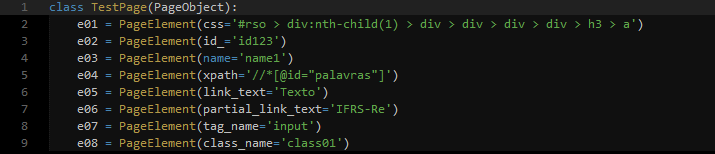
\includegraphics[width=1\textwidth]{./04-figuras/selectors}
                \label{fig:selectors}
            \end{figure}
            \vspace*{-0,9cm}
            {\raggedright \fonte{Autor desta monografia, 2017.}}

        \subsection{PageObject}
            Classe simbólica, serve apenas para poder juntar diversos PageElement descritos pelo usuário em uma classe para melhor
            legibilidade e componentização das páginas mapeadas.



    \section{Report}

        Estes módulo está destinado para geração de logs de execuções internas do \emph{framework}, criação e controle
        de logs definidos pelos usuário e a criação de planilhas analíticas de dados extraídos das páginas.

        \subsection{Logger}
        Classe de geração dos Logs de execução do \emph{framework}, onde cada execução, ação, sucessos e falhas podem ser configurados para que no decorrer do processo
        sejam mostrados no terminal de execução e no final salvos em um arquivo de texto.

        Na \autoref{fig:logs} podemos verificar 2 tipos de escritas do \emph{log}, onde na linha 11 temos a escrita de um \emph{log} e na linha 21 é o tratamento
        de erros de execução, onde este para a execução do codigo ao ser chamado.

        \begin{figure}[H]
            \vspace*{0,3cm}
            \centering
            \caption{Exemplo - Uso do Logger}
            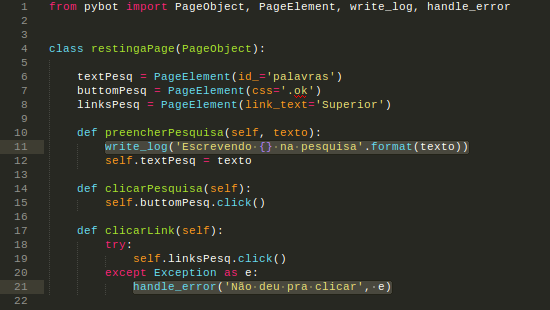
\includegraphics[width=0.9\textwidth]{./04-figuras/logs}
            \label{fig:logs}
        \end{figure}
        \vspace*{-0,9cm}
        {\raggedright \fonte{Autor desta monografia, 2017.}}

        \subsection{CsvHandler}
        Utilizado para geração de planilhas com dados extraídos das páginas para análise posterior dos usuários. Os dados tem que ser extraídos manualmente pelo
        usuário, e uma vez extraídos são salvos automaticamente em um arquivo com a extensão \emph{csv}.

        Como exemplo, podemos observar na \autoref{fig:csv} um exemplo de utilização do \emph{CsvHandler}, onde, na linha 5 será criado uma planilha contendo uma
        coluna Disciplina e na linha 21 será inserido registros na planilha abaixo da coluna.

        \begin{figure}[H]
            \vspace*{0,3cm}
            \centering
            \caption{Exemplo - Uso do CsvHandler}
            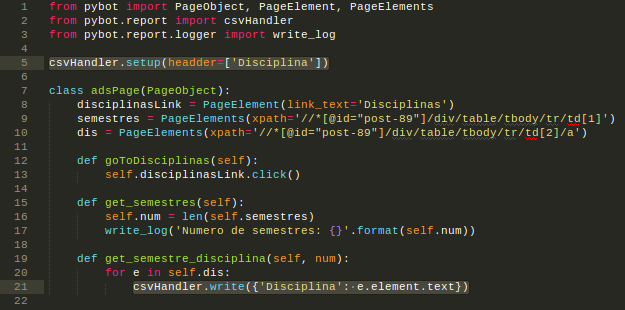
\includegraphics[width=0.9\textwidth]{./04-figuras/csv}
            \label{fig:csv}
        \end{figure}
        \vspace*{-0,9cm}
        {\raggedright \fonte{Autor desta monografia, 2017.}}

    \section{Driloader}
    \label{driloader}
        Driloader é o responsável pelo download dos \textit{drivers} de cada navegador,suportando \textit{download} dos \textit{drivers} do Internet Explorer,
        Firefox e Chrome, sendo possível para o usuário selecionar uma versão específica, a ultima versão ou detectar automaticamente qual a versão adequada para o navegador
        instalado do usuário. Como para utilização do \emph{Selenium Webdriver} é necessário um \textit{driver} específico de cada navegador foi tomada a decisão da criação
        desse projeto que inicialmente era um módulo do \emph{framework} mas pela autonomia e praticidade que ele proporciona aos usuários do Selenium Webdriver foi feita a
        separação dele do Pybot. Seu uso é feito na classe Manager(\ref{sec:manager}) automaticamente quando nenhuma \emph{driver} é encontrado no computador do usuário.



